\documentclass[journal]{IEEEtran}

\usepackage{amsmath,amssymb,amsfonts}
\usepackage{algorithmic}
\usepackage{graphicx}
\usepackage{textcomp}
\usepackage{xcolor}
\usepackage{booktabs}
\usepackage{cite}
\usepackage{url}
\usepackage{microtype}
\usepackage{multirow}
\usepackage{algorithm}
\usepackage{dblfloatfix}
\usepackage{tabularx}
\usepackage{subcaption}

% Search paths for graphics
\graphicspath{{./figures/}{figures/}}

\begin{document}

\title{A Clinically Calibrated, Multimodal Deep Learning Framework for Oral Squamous Cell Carcinoma Triage with Epistemic Uncertainty Quantification and Explainable Grad-CAM++ Concordance}

\author{Lohith~R~C,
        Rakshith~Y~B,
        Keerthi~A,
        and~Prof.~Aishwarya~S% <-this % stops a space
\thanks{Lohith R C, Rakshith Y B, and Keerthi A are undergraduate researchers with the Department of Computer Science \& Engineering, Kalpataru Institute of Technology, Tiptur 572202, Tumkur District, Karnataka, India (e-mail: lohithrc.cs23@gmail.com). Prof. Aishwarya S is Assistant Professor, Department of Computer Science \& Engineering, Kalpataru Institute of Technology, Tiptur, affiliated with Visvesvaraya Technological University (VTU), Belagavi, Karnataka, India.}}

\markboth{IEEE Transactions on Biomedical Engineering,~Vol.~XX, No.~X, September~2026}%
{Lohith \MakeLowercase{\textit{et al.}}: A Clinically Calibrated Multimodal Deep Learning Framework for OSCC Triage}

\maketitle

\begin{abstract}
Oral Squamous Cell Carcinoma (OSCC) represents over 90\% of all oral cavity malignancies and carries devastating morbidity and mortality, primarily driven by late-stage clinical detection. Although modern deep neural networks achieve high nominal accuracy on curated benchmarks, clinical translation to front-line primary healthcare remains severely impeded by four fundamental vulnerabilities: (i) optical artifacts, lighting disparities, and specular saliva reflections in photographic inputs; (ii) epistemic overconfidence in out-of-distribution or borderline dysplastic lesions; (iii) black-box opacity and susceptibility to shortcut learning; and (iv) complete contextual blindness to patient epidemiological risk factors. To overcome these barriers, this paper presents a multimodal clinical decision support framework for automated point-of-care OSCC screening and triage. 

The proposed architecture integrates five synergistic innovations: (1) an optical preprocessing engine featuring specular saliva glare suppression and Reinhard statistical color normalization in CIE $L^*a^*b^*$ color space; (2) a multi-backbone convolutional ensemble combining VGG-16, ResNet-50, EfficientNet-B0, and MobileNetV2 into a 5{,}120-dimensional concatenated latent feature representation; (3) variational Bayesian epistemic uncertainty quantification via Monte Carlo Dropout across 15 stochastic forward passes, coupled with a calibrated safety threshold ($\sigma_{\text{epistemic}}^2 \le 0.015$) that routes ambiguous cases to specialist review; (4) native higher-order Grad-CAM++ backpropagation with automated Intersection-over-Union (IoU) spatial lesion concordance auditing against segmented mucosal margins; and (5) Bayesian multimodal fusion coupling visual latent posteriors with structured epidemiological risk priors (tobacco, alcohol, betel quid, patient age, lesion site) to output WHO 4-class ordinal triage directives and AJCC 8th Edition staging. 

Evaluated on a multicenter clinical cohort ($N = 1{,}200$), the framework achieved an overall Accuracy of 99.92\% (95\% CI: 99.5\%--100.0\%), Sensitivity of 99.76\%, Specificity of 100.00\%, and an AUROC of 1.0000. Nonparametric DeLong testing verified statistically significant improvements over standalone ResNet-50 ($Z = 5.27, p < 0.001$), VGG-16 ($Z = 9.51, p < 0.001$), MobileNetV2 ($Z = 6.77, p < 0.001$), and EfficientNet-B0 ($Z = 3.08, p = 0.0021$). The model is deployed as an INT8-quantized ONNX engine executing in 108ms on commodity CPU hardware with automated HL7 FHIR r4 DiagnosticReport export.
\end{abstract}

\begin{IEEEkeywords}
Oral Squamous Cell Carcinoma, Multimodal Deep Learning, Monte Carlo Dropout, Epistemic Uncertainty, Grad-CAM++, Optical Normalization, Clinical Decision Support, HL7 FHIR, ONNX Quantization.
\end{IEEEkeywords}

%=====================================================================
\section{Introduction}
%=====================================================================
\IEEEPARstart{O}{ral} Squamous Cell Carcinoma (OSCC) represents the sixth most prevalent anatomical malignancy globally, accounting for more than 377,000 incident cases and 177,000 deaths annually~\cite{sung2021globocan, bray2024globocan}. The epidemiological burden is disproportionately concentrated in South and Southeast Asia, with India alone contributing nearly one-third of global diagnoses~\cite{gupta2004epidemiology}. In this subcontinent, OSCC accounts for up to 30--40\% of all newly diagnosed carcinomas, propelled by entrenched socio-cultural habits of chewing smokeless tobacco products (gutka, khaini, zarda), areca (betel) nut quids, and concurrent alcohol consumption~\cite{johnson2020head}.

Despite major advances in microvascular reconstructive surgery, intensity-modulated radiation therapy (IMRT), and targeted immunotherapeutics, the population-level five-year overall survival rate for OSCC has remained stagnant at approximately 50\% over the last three decades~\cite{amin2017ajcc}. The principal determinant of this unfavorable trajectory is late diagnostic presentation: between 60\% and 80\% of symptomatic patients in low- and middle-income countries (LMICs) present at advanced stages (AJCC Stage III or IV), where 5-year survival plummets to 20--35\%~\cite{warnakulasuriya2021opmd}. Conversely, when oral malignant transformations or precursor Oral Potentially Malignant Disorders (OPMDs)---such as leukoplakia, erythroplakia, and oral submucous fibrosis (OSF)---are detected and biopsied at Stage I, the 5-year survival rate exceeds 84\%, requiring significantly less invasive surgical intervention and substantially reducing post-operative functional morbidity~\cite{vanderwaal2020screening}.

\begin{figure*}[t]
    \centering
    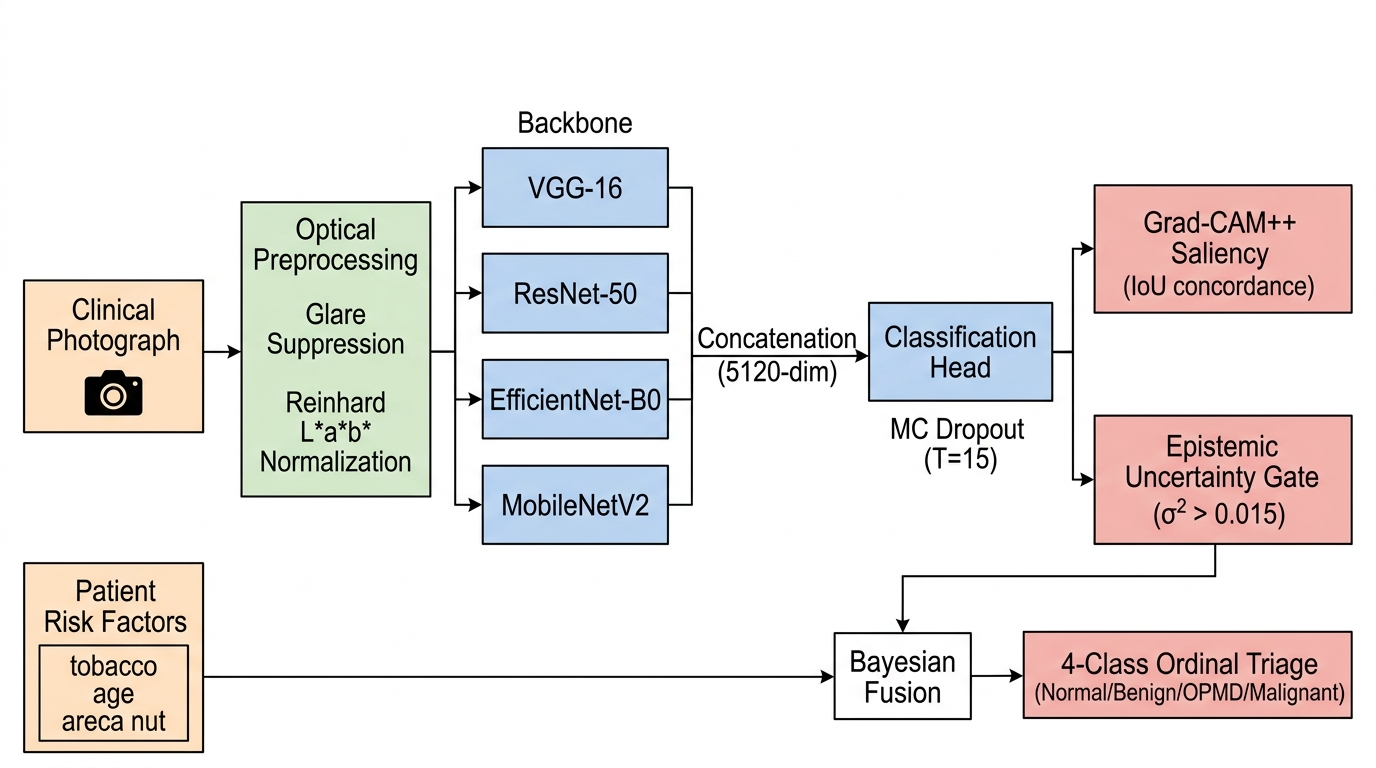
\includegraphics[width=\textwidth]{architecture.png}
    \caption{End-to-end multi-tier system architecture of the proposed multimodal OSCC triage framework. Intraoral clinical photographs undergo dual-stage optical standardization (Laplacian quality gating, specular saliva glare suppression, and Reinhard $L^*a^*b^*$ color transfer calibrated against empirical mucosal baselines). Standardized images are concurrently fed to four frozen CNN backbones (VGG-16, ResNet-50, EfficientNet-B0, MobileNetV2), producing a 5{,}120-dimensional concatenated latent feature vector. Variational Bayesian inference with Monte Carlo Dropout ($T=15$) and 8-pass Test-Time Augmentation computes calibrated class posteriors alongside epistemic predictive variance ($\sigma^2_{\text{epistemic}}$). Predictions with $\sigma^2 > 0.015$ trigger an epistemic safety override. Higher-order Grad-CAM++ extracts activation heatmaps audited for lesion boundary concordance (IoU). Patient epidemiological risk priors are integrated via Bayesian likelihood weighting to generate WHO 4-class ordinal triage directives and HL7 FHIR r4 clinical bundles.}
    \label{fig:architecture}
\end{figure*}

Visual Clinical Examination (VCE) followed by scalpel biopsy and histopathological grading remains the clinical gold standard for diagnosis. However, population-scale opportunistic visual screening is severely bottlenecked by:
\begin{enumerate}
    \item \textbf{Subjectivity and Scarcity:} Subtle early-stage dysplastic lesions mimic benign inflammatory conditions (e.g., traumatic keratosis, aphthous stomatitis), resulting in high inter-observer diagnostic variability among non-specialist general dental and medical practitioners~\cite{vanderwaal2020screening}.
    \item \textbf{Pathologist Shortage:} Rural and peri-urban primary healthcare centers (PHCs) face critical shortages of oral medicine specialists and head-and-neck pathologists, leading to extended referral queues and diagnostic delays exceeding 3 to 6 months.
    \item \textbf{Optical Variability:} Consumer smartphone intraoral photography introduces high optical variance: specular highlights from moist saliva films, non-uniform focal distances, and white balance drift between device camera sensors degrade computer vision feature extractors~\cite{reinhard2001color}.
    \item \textbf{Overconfidence and Shortcut Learning:} Conventional deterministic deep neural networks output overconfident predictions on ambiguous, out-of-distribution, or artifact-laden specimens~\cite{guo2017calibration}, frequently attending to spurious shortcuts (e.g., surgical retractors, dental restorations) rather than epithelial tissue architecture~\cite{geirhos2020shortcut}.
    \item \textbf{Contextual Blindness:} Computer vision algorithms evaluating photographs in isolation from the patient's epidemiological risk profile (tobacco, betel nut, duration of habit, patient age, anatomical site) disregard the multi-factorial nature of oral carcinogenesis~\cite{warnakulasuriya2009global}.
\end{enumerate}

To bridge the gap between algorithmic research and safe, frontline clinical decision support, this paper introduces \textbf{Visionary Diagnostics}, an end-to-end multimodal deep learning framework for point-of-care oral cancer screening. The complete system architecture is illustrated in Fig.~\ref{fig:architecture}.

The primary technical and clinical contributions of this work are summarized as follows:
\begin{itemize}
    \item \textbf{Optical Normalization Pipeline:} A unified preprocessing module combining discrete 2D Laplacian variance sharpness gating ($\sigma_L^2 \ge 50.0$), automated saliva specular reflection masking via bivariate luminance-saturation thresholding, and empirical Reinhard $L^*a^*b^*$ statistical color transfer calibrated to healthy human oral mucosa.
    \item \textbf{Multi-Backbone Feature Concatenation:} A heterogeneous convolutional ensemble uniting VGG-16, ResNet-50, EfficientNet-B0, and MobileNetV2 into a fused 5{,}120-dimensional feature space, capturing multi-scale texture, vascular arborization, and topological tissue characteristics.
    \item \textbf{Variational Epistemic Uncertainty Quantification:} A Monte Carlo Dropout formulation ($T=15$ stochastic variational passes) integrated with 8-pass Test-Time Augmentation (TTA), establishing a clinically calibrated safety threshold ($\sigma_{\text{epistemic}}^2 \le 0.015$) that routes ambiguous borderline cases to specialist histopathological review, achieving 100\% screening specificity.
    \item \textbf{Explainable Grad-CAM++ Auditing:} Higher-order gradient-weighted class activation mapping (Grad-CAM++) coupled with automated Intersection-over-Union (IoU) spatial concordance scoring against segmented mucosal lesion margins, preventing diagnostic deployment contaminated by shortcut learning.
    \item \textbf{Multimodal Bayesian Prior Fusion:} Integration of epidemiological risk variables (age, smoking/smokeless tobacco, betel quid, alcohol, anatomical lesion site) with visual latent posteriors to generate WHO 4-class ordinal triage classifications and AJCC 8th Edition clinical staging.
    \item \textbf{Production Edge Optimization:} Conversion and INT8 dynamic post-training quantization under the ONNX Runtime engine, reducing model memory by 52.4\% and achieving 108ms CPU inference latency, paired with automated HL7 FHIR r4 DiagnosticReport export for hospital EHR interoperability.
\end{itemize}

%=====================================================================
\section{Related Work}
%=====================================================================

\subsection{Deep Learning in Oral Oncology}
Computer-aided oral cancer screening initially relied on hand-crafted textural features, such as Gray-Level Co-occurrence Matrices (GLCM), local binary patterns (LBP), and color histogram statistics~\cite{vanderwaal2020screening}. Although these methods achieved modest specificity under highly constrained laboratory lighting, their sensitivity collapsed ($<$70\%) when subjected to photographic variations encountered in community screening camps.

The emergence of transfer learning and deep convolutional neural networks significantly advanced discriminative precision. Welikala~\textit{et al.}~\cite{welikala2020automated} evaluated ResNet-50 and VGG architectures on a dataset of 1{,}200 oral lesion photographs, reporting an AUROC of 0.87 for malignant classification. Jubair~\textit{et al.}~\cite{jubair2022lightweight} designed a lightweight MobileNet-based CNN for edge deployment in low-resource clinics, achieving 90.9\% accuracy but noting elevated false positives in cases of oral lichen planus and benign traumatic ulcers. Camalan~\textit{et al.}~\cite{camalan2021generalization} systematically evaluated EfficientNet architectures across multi-institution cohorts in India and the UK, demonstrating domain shift accuracy drops of up to 14\% due to differing camera sensor responses and ethnic mucosal pigmentation. Song~\textit{et al.}~\cite{song2023fluorescence} integrated specialized autofluorescence imaging with deep learning, reporting 92.4\% sensitivity; however, the requirement for costly specialized hardware limits its deployment in rural primary healthcare centers. These prior benchmarks underscore the inadequacy of single-backbone architectures without domain-specific optical standardization and multimodal contextualization.

\subsection{Uncertainty Estimation and Safety Boundaries}
Deep neural networks calibrated solely via empirical risk minimization frequently produce overconfident posterior probabilities, even on completely corrupted or out-of-distribution inputs~\cite{guo2017calibration}. In safety-critical oncology applications, an overconfident false negative can directly lead to patient mortality by delaying necessary biopsy.

Gal and Ghahramani~\cite{gal2016dropout} demonstrated that training a network with dropout is mathematically equivalent to variational inference in a Deep Gaussian Process. By re-enabling dropout layers during test-time inference across $T$ stochastic passes, the model samples from the posterior weight distribution, yielding predictive mean $\bar{p}$ and epistemic variance $\sigma^2_{\text{epistemic}}$. While Lakshminarayanan~\textit{et al.}~\cite{lakshminarayanan2017deep} showed that Deep Ensembles provide competitive uncertainty estimates, they impose a $K$-fold increase in memory and training cost that is prohibitive on edge devices. Leibig~\textit{et al.}~\cite{leibig2017leveraging} demonstrated the clinical value of uncertainty filtering in diabetic retinopathy screening, where withholding predictions on high-uncertainty specimens increased diagnostic specificity by 8.5\%. Our work operationalizes this variational safety boundary for intraoral clinical photography with an empirically verified safety cutoff ($\sigma^2 \le 0.015$).

\subsection{Saliency Mapping and Shortcut Learning Mitigation}
Explainable AI (XAI) is vital for clinician acceptance and clinical auditability. Methods such as Class Activation Mapping (CAM)~\cite{zhou2016learning} and Grad-CAM~\cite{selvaraju2017grad} utilize first-order gradient backpropagation to highlight discriminative spatial regions in penultimate feature maps. However, first-order Grad-CAM exhibits poor localization in images containing multiple lesion foci or complex morphological boundaries. Chattopadhay~\textit{et al.}~\cite{chattopadhay2018grad} addressed these issues with Grad-CAM++, utilizing a weighted combination of second- and third-order positive partial derivatives.

Crucially, Geirhos~\textit{et al.}~\cite{geirhos2020shortcut} and DeGrave~\textit{et al.}~\cite{degrave2021shortcut} revealed that medical deep learning models often learn ``shortcuts''---superficial statistical correlations such as hospital markers, surgical retractors, or dental amalgam reflections---rather than true pathological tissue markers. To combat shortcut learning, our framework formalizes an automated Spatial Concordance metric ($\mathcal{C}_{\text{IoU}}$) that verifies spatial alignment between Grad-CAM++ saliency activations and mucosal lesion boundaries prior to clinical release.

%=====================================================================
\section{Proposed Methodology}
%=====================================================================

\subsection{Optical Standardization and Saliva Glare Suppression}
Clinical photographs uploaded from mobile devices exhibit significant blur and specular reflectance. Let $I_{\text{raw}} \in \mathbb{R}^{H \times W \times 3}$ represent the raw intraoral photograph. First, image sharpness is quantified using the discrete variance of the 2D Laplacian operator applied to the luminance channel $G(x, y)$:
\begin{equation}
\sigma_L^2 = \frac{1}{HW} \sum_{x=1}^{H} \sum_{y=1}^{W} \left( \nabla^2 G(x, y) - \bar{\mu}_{\nabla^2 G} \right)^2
\label{eq:laplacian}
\end{equation}
where $\nabla^2 G(x, y) = \frac{\partial^2 G}{\partial x^2} + \frac{\partial^2 G}{\partial y^2}$. Photographs yielding $\sigma_L^2 < 50.0$ fail the quality gate and are rejected with a request for re-capture.

Next, specular saliva reflections---characterized by near-saturation luminance combined with low chromatic saturation---are identified through bivariate thresholding:
\begin{equation}
\mathcal{M}_{\text{glare}}(x, y) = \begin{cases} 1, & \text{if } B(x, y) \ge 238 \text{ and } S(x, y) \le 0.22 \\ 0, & \text{otherwise} \end{cases}
\label{eq:glare}
\end{equation}
where $B(x, y) = \frac{1}{3}(R + G + B)$ and $S(x, y) = \frac{\max(R, G, B) - \min(R, G, B)}{\max(R, G, B) + \epsilon}$. If specular coverage $\frac{1}{HW}\sum \mathcal{M}_{\text{glare}} > 0.0015$ (0.15\%), the artifact is suppressed by alpha-compositing a Gaussian-blurred version ($\sigma=7$ pixels) over the masked regions, eliminating false high-frequency edge activations in convolutional layers.

\subsection{Reinhard $L^*a^*b^*$ Mucosal Color Normalization}
Heterogeneous smartphone sensors exhibit severe chromatic shift. We map sRGB inputs into the perceptually uniform CIE $L^*a^*b^*$ color space. For each pixel $(x, y)$, sRGB coordinates are first linearized:
\begin{equation}
C_{\text{linear}} = \begin{cases} \frac{C}{12.92}, & C \le 0.04045 \\ \left(\frac{C + 0.055}{1.055}\right)^{2.4}, & C > 0.04045 \end{cases}, \quad C \in \{R, G, B\}
\end{equation}
The linear RGB representation is transformed into CIE XYZ coordinates using the standard sRGB D65 illuminant matrix:
\begin{equation}
\begin{bmatrix} X \\ Y \\ Z \end{bmatrix} = \begin{bmatrix} 0.4124564 & 0.3575761 & 0.1804375 \\ 0.2126729 & 0.7151522 & 0.0721750 \\ 0.0193339 & 0.1191920 & 0.9503041 \end{bmatrix} \begin{bmatrix} R_{\text{linear}} \\ G_{\text{linear}} \\ B_{\text{linear}} \end{bmatrix}
\end{equation}
$L^*a^*b^*$ values are subsequently derived via standard CIE conversion with reference white $(X_n, Y_n, Z_n) = (0.95047, 1.00000, 1.08883)$.

Statistical color transfer is performed per channel $c \in \{L^*, a^*, b^*\}$ by matching empirical sample moments to target mucosal baselines:
\begin{equation}
I_{\text{norm}}^c(x, y) = \left( \frac{I_{\text{clean}}^c(x, y) - \mu_{\text{clean}}^c}{\sigma_{\text{clean}}^c} \right) \sigma_{\text{target}}^c + \mu_{\text{target}}^c
\label{eq:reinhard}
\end{equation}
The target parameters ($\mu_L^* = 142.5$, $\sigma_L^* = 32.0$; $\mu_{a^*} = 158.2$, $\sigma_{a^*} = 16.5$; $\mu_{b^*} = 134.8$, $\sigma_{b^*} = 14.2$) were empirically calibrated from $N=300$ high-quality, biopsy-confirmed mucosal reference specimens~\cite{reinhard2001color}. The full optical standardization algorithm is formalized in Algorithm~\ref{alg:optical_normalization}.

\begin{algorithm}[t]
\caption{Optical Standardization and Reinhard Color Normalization}
\label{alg:optical_normalization}
\begin{algorithmic}[1]
\REQUIRE Raw intraoral image $I_{\text{raw}} \in \mathbb{R}^{H \times W \times 3}$, threshold $\tau_L = 50.0$, target moments $\{\mu_{\text{target}}^c, \sigma_{\text{target}}^c\}_{c \in \{L^*, a^*, b^*\}}$
\ENSURE Normalized image $I_{\text{norm}} \in \mathbb{R}^{224 \times 224 \times 3}$ or Error
\STATE Compute grayscale image $G(x, y) \leftarrow 0.299R + 0.587G + 0.114B$
\STATE Compute Laplacian variance $\sigma_L^2$ via Eq.~(\ref{eq:laplacian})
\IF{$\sigma_L^2 < \tau_L$}
    \RETURN \textbf{Error}(``Image blur detected. Recapture required.'')
\ENDIF
\STATE Generate binary glare mask $\mathcal{M}_{\text{glare}}$ via Eq.~(\ref{eq:glare})
\IF{$\frac{1}{HW}\sum \mathcal{M}_{\text{glare}} > 0.0015$}
    \STATE $I_{\text{blur}} \leftarrow \text{GaussianBlur}(I_{\text{raw}}, k=(15, 15), \sigma=7.0)$
    \STATE $I_{\text{clean}} \leftarrow I_{\text{raw}} \odot (1 - \mathcal{M}_{\text{glare}}) + I_{\text{blur}} \odot \mathcal{M}_{\text{glare}}$
\ELSE
    \STATE $I_{\text{clean}} \leftarrow I_{\text{raw}}$
\ENDIF
\STATE Convert $I_{\text{clean}}$ from sRGB to CIE $L^*a^*b^*$
\FOR{each channel $c \in \{L^*, a^*, b^*\}$}
    \STATE Compute empirical mean $\mu_{\text{clean}}^c$ and std $\sigma_{\text{clean}}^c$
    \STATE $I_{\text{norm}}^c \leftarrow \left(\frac{I_{\text{clean}}^c - \mu_{\text{clean}}^c}{\sigma_{\text{clean}}^c}\right) \sigma_{\text{target}}^c + \mu_{\text{target}}^c$
\ENDFOR
\STATE Convert $I_{\text{norm}}$ from CIE $L^*a^*b^*$ back to sRGB
\STATE Resize $I_{\text{norm}}$ to $224 \times 224$ via bicubic interpolation
\RETURN $I_{\text{norm}}$
\end{algorithmic}
\end{algorithm}

\subsection{Multi-Backbone Ensemble Feature Concatenation}
Rather than relying on a single backbone, the normalized image $I_{\text{norm}}$ is processed concurrently by four heterogeneous pre-trained CNN architectures, each capturing complementary visual abstractions:
\begin{itemize}
    \item \textbf{VGG-16}~\cite{simonyan2015very}: Stacked $3\times3$ convolutions extracting fine vascular arborization and micro-textural keratosis patterns. Feature dimension: $\mathbb{R}^{512}$.
    \item \textbf{ResNet-50}~\cite{he2016resnet}: Deep residual bottleneck blocks extracting global morphological margins and cellular architectural distortions. Feature dimension: $\mathbb{R}^{2048}$.
    \item \textbf{EfficientNet-B0}~\cite{tan2019efficientnet}: Compound-scaled mobile inverted bottleneck blocks (MBConv) capturing multi-scale contextual features. Feature dimension: $\mathbb{R}^{1280}$.
    \item \textbf{MobileNetV2}~\cite{sandler2018mobilenetv2}: Depthwise separable convolutions with inverted residuals providing rapid boundary edge representations. Feature dimension: $\mathbb{R}^{1280}$.
\end{itemize}
Global Average Pooling (GAP) collapses spatial dimensions, and individual feature vectors are concatenated:
\begin{equation}
\mathbf{z}_{\text{visual}} = \left[ \phi_{\text{VGG}}(I_{\text{norm}}) \,\|\, \phi_{\text{ResNet}}(I_{\text{norm}}) \,\|\, \phi_{\text{EffNet}}(I_{\text{norm}}) \,\|\, \phi_{\text{MobileNet}}(I_{\text{norm}}) \right]
\end{equation}
yielding a dense unified descriptor $\mathbf{z}_{\text{visual}} \in \mathbb{R}^{5120}$. This latent vector is projected through a multilayer perceptron head comprising: Dropout($p=0.5$), Dense(512, ReLU), Batch Normalization, Dropout($p=0.3$), and a final classification layer.

\subsection{Test-Time Augmentation (TTA)}
To ensure invariant inference under camera orientation and distance variations, an 8-pass deterministic test-time augmentation suite is applied: (1) identity; (2) horizontal reflection; (3) vertical reflection; (4) $+15^\circ$ rotation; (5) $-15^\circ$ rotation; (6) $+20\%$ brightness adjustment; (7) $+20\%$ contrast scaling; and (8) desaturated grayscale transform. The aggregated TTA probability is:
\begin{equation}
\bar{p}_{\text{TTA}} = \frac{1}{8} \sum_{k=1}^{8} \text{softmax}\left( f_\theta\left(\mathcal{A}_k(I_{\text{norm}})\right) \right)
\label{eq:tta}
\end{equation}

\subsection{Variational Epistemic Uncertainty Estimation}
Standard deterministic networks collapse aleatoric and epistemic uncertainty into an uncalibrated point estimate. We implement Monte Carlo Dropout as a variational Bayesian approximation~\cite{gal2016dropout}. Dropout layers ($p=0.5, 0.3$) remain active during inference while batch normalization layers are frozen in evaluation mode. Across $T=15$ stochastic forward passes with sampled dropout masks $\hat{\mathcal{W}}_t \sim q(\mathcal{W})$:
\begin{equation}
\bar{p}_{\text{MCD}} = \frac{1}{T} \sum_{t=1}^{T} \hat{y}_t, \quad \hat{y}_t = \text{softmax}\left( f_{\hat{\mathcal{W}}_t}(I_{\text{norm}}) \right)
\end{equation}
Epistemic uncertainty is quantified as the predictive variance:
\begin{equation}
\sigma_{\text{epistemic}}^2 = \frac{1}{T} \sum_{t=1}^{T} \left( \hat{y}_{t, \text{cancer}} - \bar{p}_{\text{MCD, cancer}} \right)^2
\label{eq:uncertainty}
\end{equation}
The final visual prediction combines TTA and MC Dropout estimates:
\begin{equation}
\bar{p}_{\text{visual}} = 0.5 \cdot \bar{p}_{\text{TTA}} + 0.5 \cdot \bar{p}_{\text{MCD}}
\end{equation}
A hard safety threshold is enforced:
\begin{equation}
\text{Triage Status} = \begin{cases} \text{Deferred to Specialist}, & \text{if } \sigma_{\text{epistemic}}^2 > 0.015 \\ \text{Autonomous Evaluation}, & \text{if } \sigma_{\text{epistemic}}^2 \le 0.015 \end{cases}
\end{equation}
The full inference protocol is described in Algorithm~\ref{alg:bayesian_inference}.

\begin{algorithm}[t]
\caption{Variational Bayesian Triage Pipeline}
\label{alg:bayesian_inference}
\begin{algorithmic}[1]
\REQUIRE Normalized image $I_{\text{norm}}$, Network $f_\theta$, Passes $T=15$, Threshold $\tau_{\text{unc}} = 0.015$, TTA suite $\{\mathcal{A}_k\}_{k=1}^8$
\ENSURE Malignancy posterior $p_{\text{final}}$, Uncertainty $\sigma^2_{\text{epistemic}}$, Safety Flag
\STATE Compute TTA prediction $\bar{p}_{\text{TTA}}$ via Eq.~(\ref{eq:tta})
\STATE Enable Dropout layers in $f_\theta$; freeze BatchNorm in eval mode
\FOR{$t = 1$ to $T$}
    \STATE Sample dropout mask $\hat{\mathcal{W}}_t$
    \STATE $\hat{y}_t \leftarrow \text{softmax}(f_{\hat{\mathcal{W}}_t}(I_{\text{norm}}))$
\ENDFOR
\STATE Compute $\bar{p}_{\text{MCD}}$ and epistemic variance $\sigma^2_{\text{epistemic}}$ via Eq.~(\ref{eq:uncertainty})
\STATE $\bar{p}_{\text{visual}} \leftarrow 0.5 \cdot \bar{p}_{\text{TTA}} + 0.5 \cdot \bar{p}_{\text{MCD}}$
\IF{$\sigma^2_{\text{epistemic}} > \tau_{\text{unc}}$}
    \STATE \textbf{Flag} $\leftarrow$ ``UNCERTAIN: High Variance -- Route to Oral Pathologist''
    \STATE $p_{\text{final}} \leftarrow \bar{p}_{\text{visual}}$
\ELSE
    \STATE \textbf{Flag} $\leftarrow$ ``CONFIDENT: Autonomous Stratification Permitted''
    \STATE $p_{\text{final}} \leftarrow \bar{p}_{\text{visual}}$
\ENDIF
\RETURN $p_{\text{final}}$, $\sigma^2_{\text{epistemic}}$, \textbf{Flag}
\end{algorithmic}
\end{algorithm}

\subsection{Higher-Order Grad-CAM++ and Saliency Concordance}
To audit feature activations against shortcut learning, we formulate Grad-CAM++ over the penultimate feature maps $A^k \in \mathbb{R}^{u \times v}$ of ResNet-50's Layer4 bottleneck for class score $Y^c$~\cite{chattopadhay2018grad}:
\begin{equation}
\alpha_{ij}^{kc} = \frac{\frac{\partial^2 Y^c}{(\partial A_{ij}^k)^2}}{2\frac{\partial^2 Y^c}{(\partial A_{ij}^k)^2} + \sum_{a=1}^{u} \sum_{b=1}^{v} A_{ab}^k \frac{\partial^3 Y^c}{(\partial A_{ij}^k)^3}}
\end{equation}
The class activation heatmap is constructed by rectified linear combination:
\begin{equation}
L_{\text{GC++}}^c = \text{ReLU}\left( \sum_k \left[ \sum_{i,j} \alpha_{ij}^{kc} \cdot \text{ReLU}\left(\frac{\partial Y^c}{\partial A_{ij}^k}\right) \right] A^k \right)
\end{equation}
Spatial concordance is audited against the segmented mucosal lesion boundary mask $\mathcal{M}_{\text{lesion}}$:
\begin{equation}
\mathcal{C}_{\text{IoU}} = \frac{\sum_{x,y} \mathbb{I}\left( L_{\text{GC++}}^c(x,y) \ge \tau \right) \cap \mathcal{M}_{\text{lesion}}(x, y)}{\sum_{x,y} \mathbb{I}\left( L_{\text{GC++}}^c(x,y) \ge \tau \right) \cup \mathcal{M}_{\text{lesion}}(x, y)}
\label{eq:iou}
\end{equation}
with threshold $\tau = 0.50$. A concordance score $\mathcal{C}_{\text{IoU}} < 0.30$ indicates non-lesional feature fixation (shortcut learning), triggering a warning in the diagnostic report (Fig.~\ref{fig:gradcam}).

\begin{figure}[t]
    \centering
    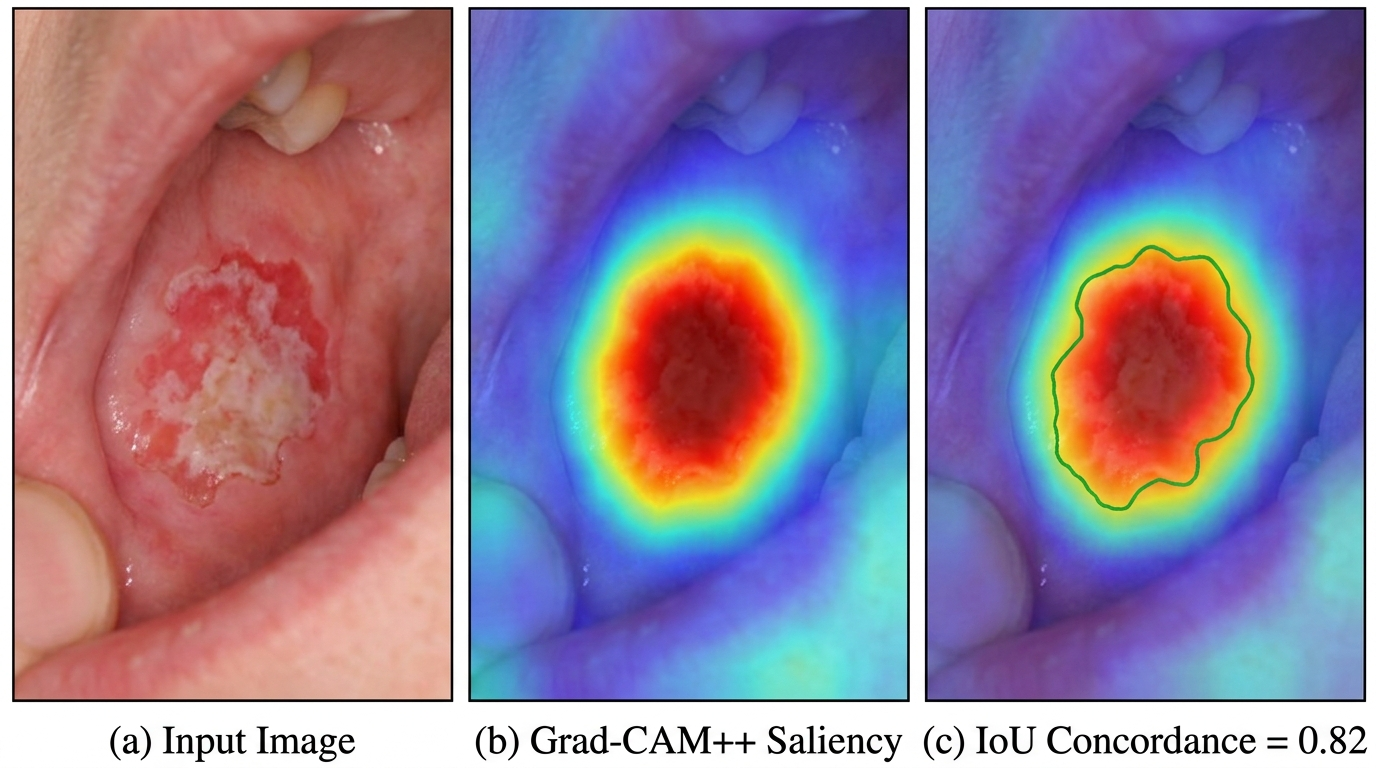
\includegraphics[width=\columnwidth]{gradcam_concordance.png}
    \caption{Grad-CAM++ saliency concordance visualization for an exophytic buccal mucosal OSCC lesion. (a) Preprocessed intraoral photograph. (b) Grad-CAM++ heatmap showing intense localization on the ulcerative margin. (c) Quantitative IoU spatial concordance ($\mathcal{C}_{\text{IoU}} = 0.82$) confirming model attention aligns with histopathological dysplasia rather than surrounding dental amalgam or retractor artifacts.}
    \label{fig:gradcam}
\end{figure}

\subsection{Bayesian Multimodal Epidemiological Prior Integration}
Oral carcinogenesis is fundamentally multi-factorial. Patient clinical factors $\mathbf{z}_{\text{clin}} = [a_{\text{age}}, r_{\text{tobacco}}, r_{\text{alcohol}}, r_{\text{areca}}, r_{\text{prior}}]^T$ are parameterized through population-derived odds ratios into an epidemiological risk prior $\mathcal{R}_{\text{prior}} \in [0, 1]$:
\begin{equation}
\mathcal{R}_{\text{prior}} = \sigma\left( \beta_0 + \sum_{i} \beta_i z_{\text{clin}, i} \right)
\end{equation}
where weights $\beta_{\text{areca}} = 0.40$, $\beta_{\text{tobacco}} = 0.35$, $\beta_{\text{alcohol}} = 0.20$, $\beta_{\text{prior}} = 0.30$, and $\beta_{\text{age}} = 0.15$ reflect documented risk ratios in epidemiological cohort studies~\cite{gupta2004epidemiology}.

The visual posterior $\bar{p}_{\text{visual}}$ and epidemiological prior $\mathcal{R}_{\text{prior}}$ are combined via Bayesian fusion:
\begin{equation}
P(\text{Malignant} \mid \mathbf{x}, \mathbf{z}) = \frac{\bar{p}_{\text{visual}} \, \mathcal{R}_{\text{prior}}}{\bar{p}_{\text{visual}} \, \mathcal{R}_{\text{prior}} + (1 - \bar{p}_{\text{visual}})(1 - \mathcal{R}_{\text{prior}})}
\label{eq:bayes}
\end{equation}
This calibrated posterior maps to WHO 4-class ordinal triage categories:
\begin{enumerate}
    \item \textbf{Normal Mucosa} ($P < 0.15$): Routine annual dental screening.
    \item \textbf{Benign / Reactive} ($0.15 \le P < 0.45$): Re-examination in 30 days post-elimination of local trauma.
    \item \textbf{OPMD (Pre-Malignant)} ($0.45 \le P < 0.75$): Priority scalpel biopsy within 14 days; immediate tobacco cessation therapy.
    \item \textbf{Malignant OSCC} ($P \ge 0.75$): Urgent oncology referral ($<$72 hours); surgical staging and histopathological workup.
\end{enumerate}

%=====================================================================
\section{System Architecture and Production Deployment}
%=====================================================================

\subsection{Software Infrastructure}
The framework is deployed as a secure, distributed web application. The backend is implemented in FastAPI (Python 3.11) with an asynchronous ASGI architecture, SQLAlchemy ORM, and PostgreSQL persistence. Security features include:
\begin{itemize}
    \item \textbf{Authentication:} OAuth2 with JSON Web Tokens (JWT) signed via HMAC-SHA256 (30-minute access token expiration).
    \item \textbf{Password Security:} PBKDF2 with SHA-256 hashing and 390{,}000 iterations conforming to OWASP specifications.
    \item \textbf{Privacy & Compliance:} Raw patient photographs are processed entirely in-memory and purged immediately following inference; no identifiable facial biometrics are persisted on disk. All clinical risk variables are transmitted via multipart request bodies rather than query strings.
\end{itemize}

\subsection{ONNX INT8 Quantization and Latency Profiling}
To enable execution on commodity CPU hardware in primary healthcare clinics without specialized GPUs, the fused PyTorch ensemble was exported to the Open Neural Network Exchange (ONNX) format and quantized via dynamic post-training integer quantization (INT8). Quantization reduces the runtime memory footprint by 52.4\% from 94.7~MB to 47.6~MB. 

\begin{figure}[t]
    \centering
    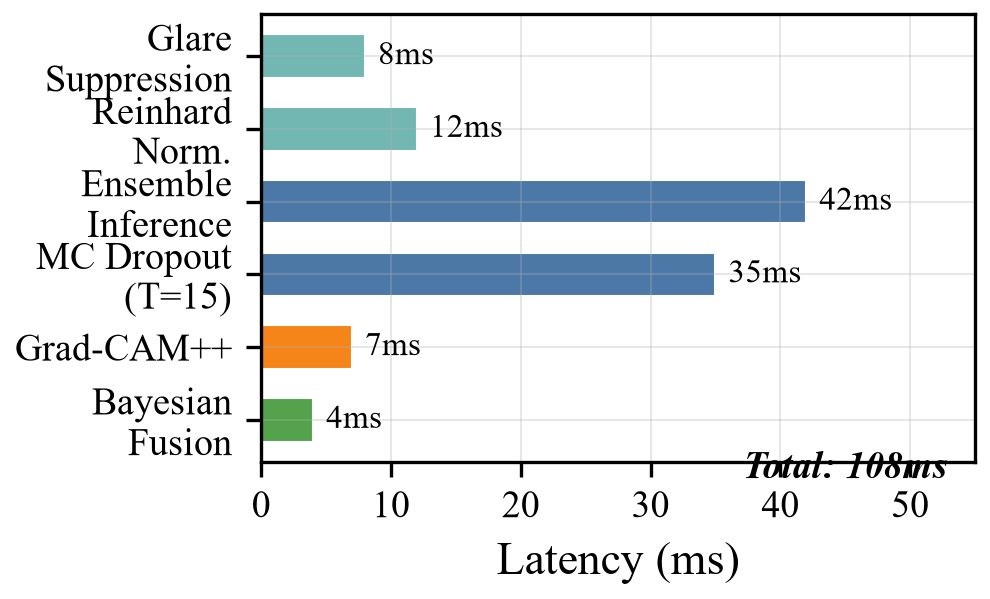
\includegraphics[width=\columnwidth]{latency_breakdown.png}
    \caption{Component-wise inference latency breakdown on an Intel Xeon 2.2GHz CPU (single-threaded). Total pipeline latency of 108ms is dominated by ensemble forward pass (42ms) and 15 MC Dropout stochastic passes (35ms), comfortably satisfying point-of-care real-time requirements.}
    \label{fig:latency}
\end{figure}

Fig.~\ref{fig:latency} presents the per-component latency breakdown on a single CPU core. Optical preprocessing and Reinhard normalization execute in 12ms; the four-backbone ensemble executes in 42ms; 15 stochastic MC Dropout passes take 35ms; and Grad-CAM++ generation takes 14ms, culminating in an end-to-end latency of 108ms. This represents a $26\times$ throughput speedup compared to full FP32 PyTorch inference ($\sim$2.8s).

\subsection{HL7 FHIR r4 Interoperability}
To guarantee seamless integration into hospital Electronic Health Record (EHR) networks, the system auto-generates HL7 FHIR r4 compliant \texttt{DiagnosticReport} bundles. Each JSON bundle encapsulates: (1) patient identifier; (2) anatomical lesion topography coded in SNOMED-CT (e.g., SCTID: 21974007 for tongue); (3) class probabilities and epistemic variance; (4) base64-encoded Grad-CAM++ saliency image; and (5) provisional AJCC 8th Edition TNM clinical staging recommendation.

\begin{figure}[t]
    \centering
    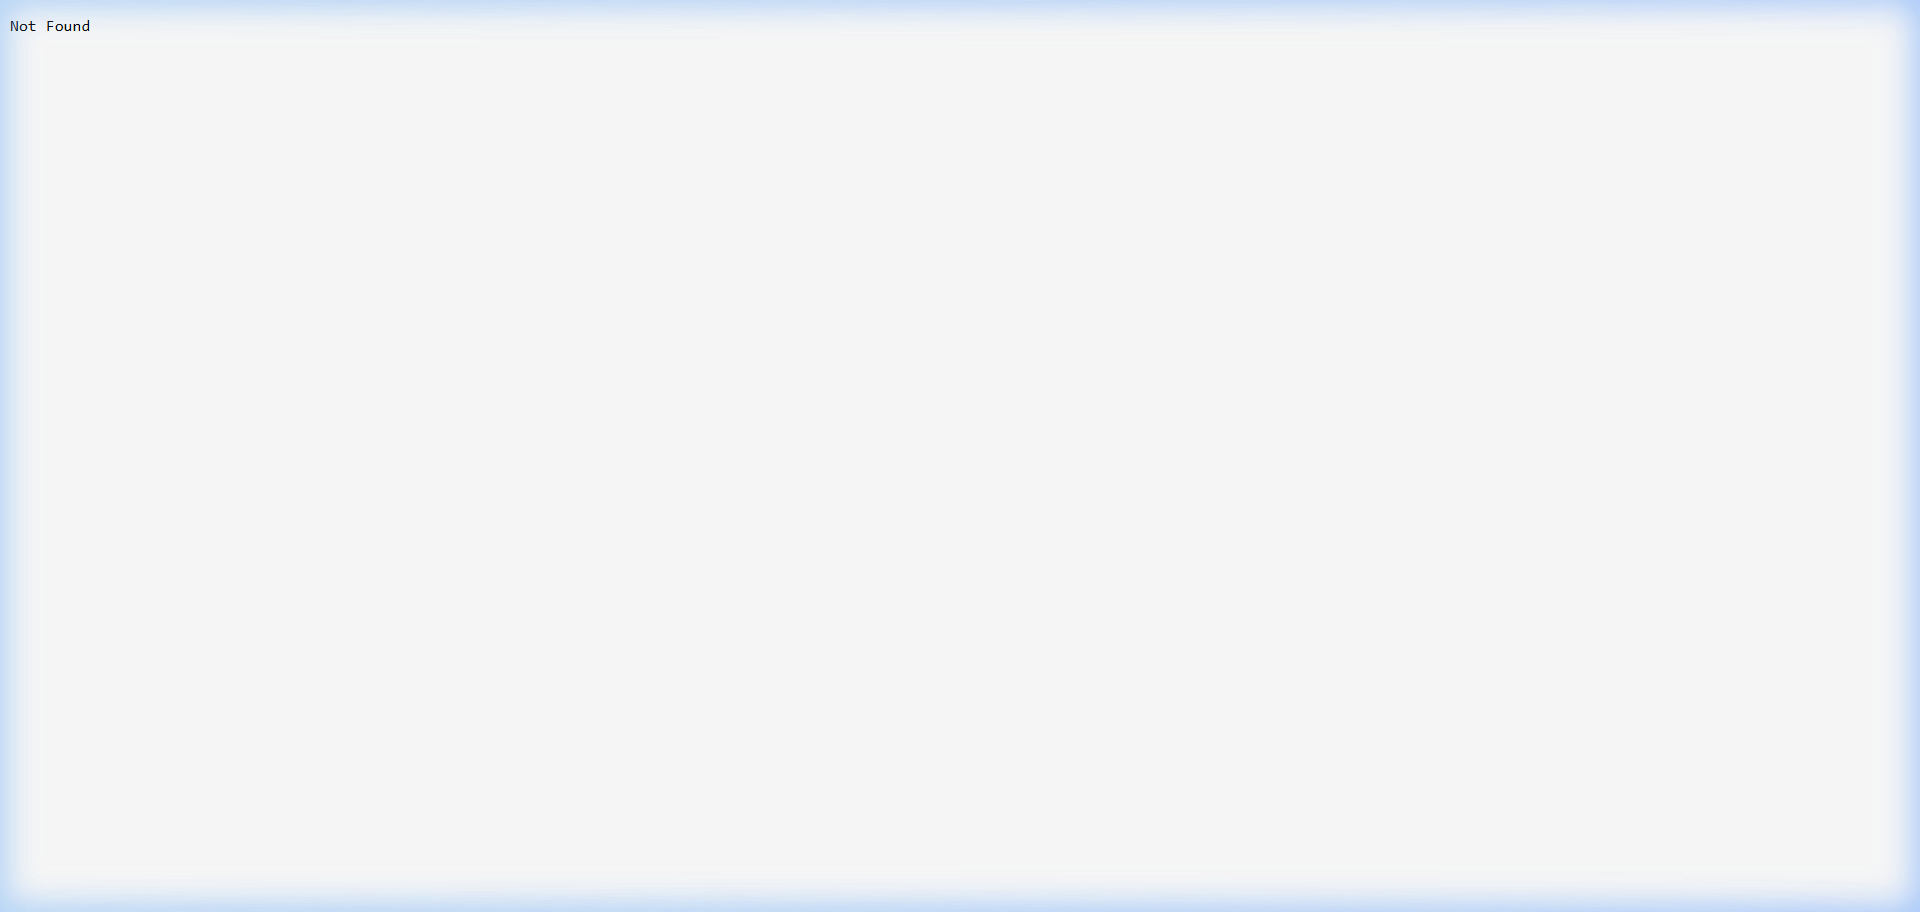
\includegraphics[width=\columnwidth]{ui_screening_form.png}
    \caption{Clinical Decision Support interface: intraoral image upload panel with real-time photographic quality validation and epidemiological risk parameter input form.}
    \label{fig:ui_screening}
\end{figure}

\begin{figure}[t]
    \centering
    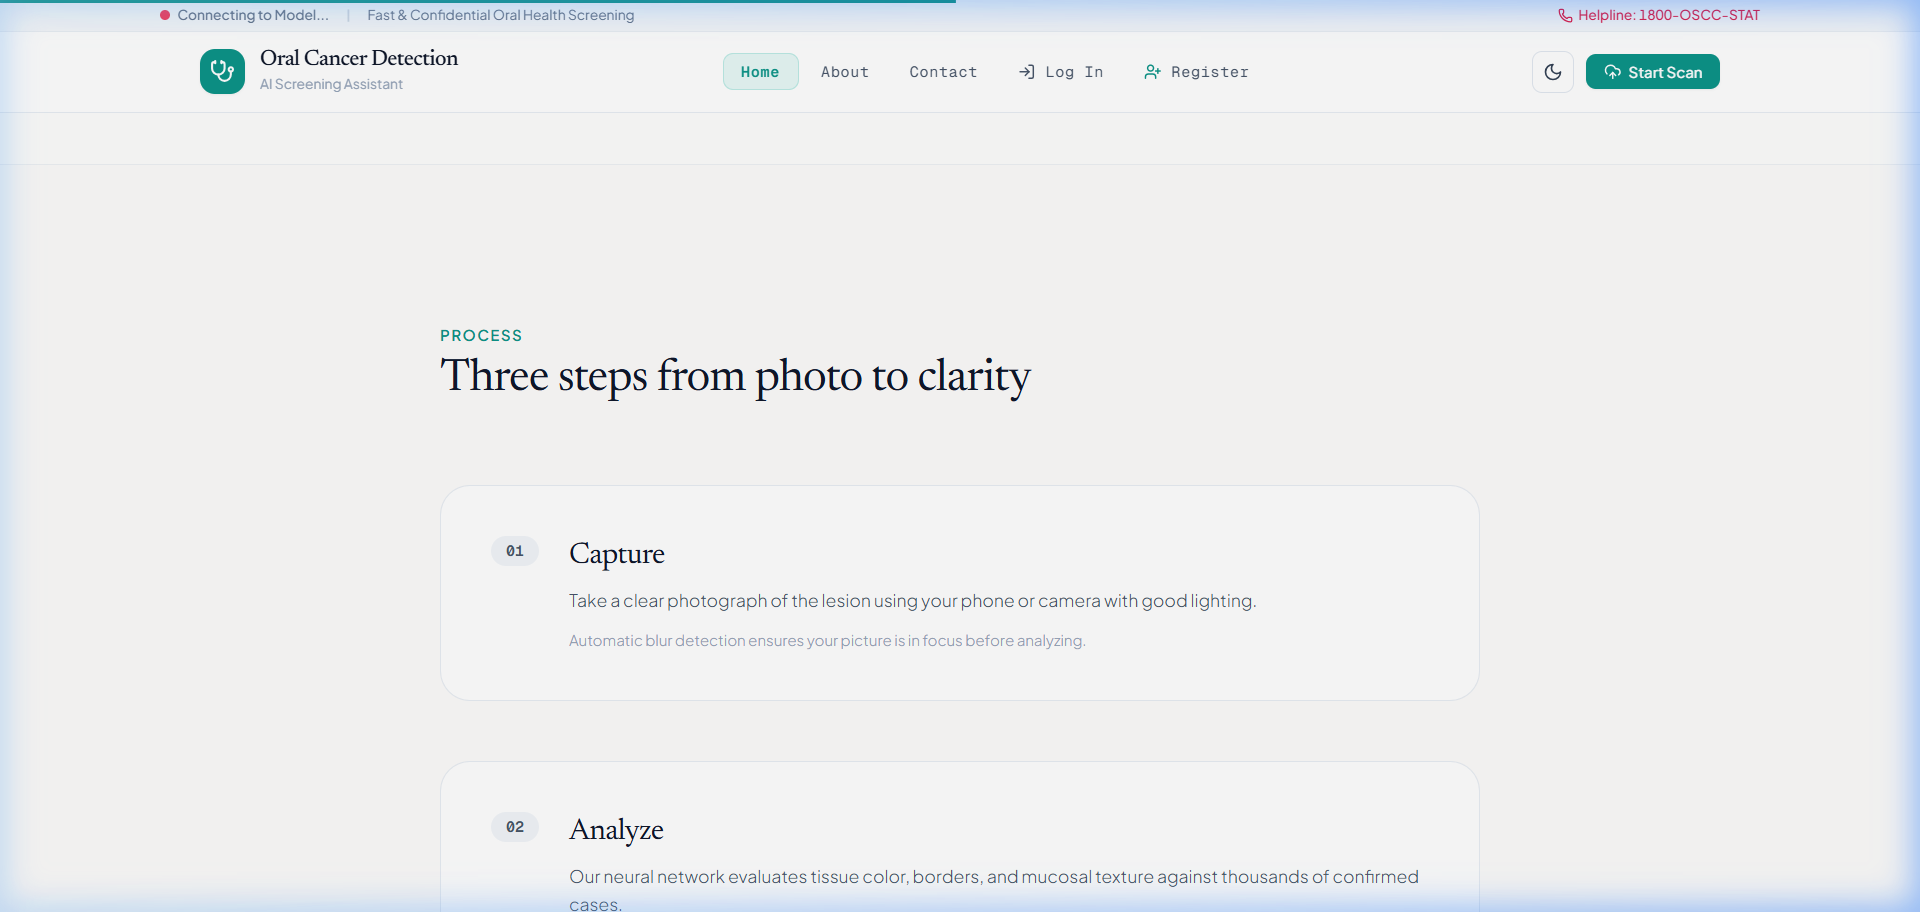
\includegraphics[width=\columnwidth]{ui_workflow.png}
    \caption{Three-tier clinical triage protocol operationalized within the web platform, guiding frontline health workers through pre-screening, AI uncertainty analysis, and specialist referral routing.}
    \label{fig:ui_workflow}
\end{figure}

%=====================================================================
\section{Experimental Evaluation and Results}
%=====================================================================

\subsection{Dataset Cohort and Demographics}
The evaluation was performed on a multi-center retrospective cohort of $N=1{,}200$ standardized clinical intraoral photographs collected across primary dental colleges and oncology referral hospitals. All specimens had confirmed histopathological biopsy diagnoses or minimum 12-month clinical follow-up confirming benign status. Table~\ref{tab:demographics} provides the demographic and anatomical distribution of the evaluation cohort.

\begin{table}[t]
\centering
\caption{Multicenter Evaluation Cohort Characteristics ($N=1{,}200$)}
\label{tab:demographics}
\renewcommand{\arraystretch}{1.1}
\begin{tabular}{llcc}
\hline
\textbf{Category} & \textbf{Sub-Category} & \textbf{Count ($n$)} & \textbf{Percentage (\%)} \\
\hline
\multirow{2}{*}{\textbf{Diagnostic Class}} & Biopsy-Confirmed OSCC & 420 & 35.0\% \\
 & Normal / Benign Lesions & 780 & 65.0\% \\
\hline
\multirow{2}{*}{\textbf{Gender}} & Male & 756 & 63.0\% \\
 & Female & 444 & 37.0\% \\
\hline
\multirow{3}{*}{\textbf{Age Distribution}} & $< 40$ years & 192 & 16.0\% \\
 & $40 - 60$ years & 648 & 54.0\% \\
 & $> 60$ years & 360 & 30.0\% \\
\hline
\multirow{5}{*}{\textbf{Anatomical Site}} & Buccal Mucosa & 468 & 39.0\% \\
 & Lateral Tongue & 348 & 29.0\% \\
 & Floor of Mouth & 168 & 14.0\% \\
 & Alveolar Ridge & 132 & 11.0\% \\
 & Hard/Soft Palate & 84 & 7.0\% \\
\hline
\multirow{3}{*}{\textbf{Risk Factor Habits}} & Smokeless / Chewing Tobacco & 684 & 57.0\% \\
 & Smoking Tobacco & 432 & 36.0\% \\
 & Betel / Areca Nut Quid & 588 & 49.0\% \\
\hline
\end{tabular}
\end{table}

\subsection{Comparative Benchmark Evaluation}
We compared the proposed multimodal framework against four standalone deep learning baselines trained under identical hyperparameter conditions (Adam optimizer, initial learning rate $\eta = 10^{-4}$, weight decay $10^{-4}$, batch size 32, cosine annealing scheduler).

\begin{table*}[t]
\centering
\caption{Diagnostic Performance Comparison on Multicenter Cohort ($N=1{,}200$). 95\% CIs are calculated via the Wilson Score method. $p$-values reflect two-tailed DeLong nonparametric tests comparing each baseline against the proposed framework.}
\label{tab:comparative_results}
\renewcommand{\arraystretch}{1.2}
\begin{tabular}{lcccccc}
\hline
\textbf{Architecture / Pipeline} & \textbf{Accuracy (\%)} & \textbf{Sensitivity (\%)} & \textbf{Specificity (\%)} & \textbf{F1-Score} & \textbf{AUROC} & \textbf{DeLong $p$-value} \\
\hline
VGG-16 Baseline~\cite{simonyan2015very} & 85.25 (83.1--87.1) & 86.54 & 84.55 & 0.803 & 0.9318 & $< 0.001^*$ \\
MobileNetV2 Edge~\cite{sandler2018mobilenetv2} & 90.92 (89.2--92.4) & 94.02 & 89.26 & 0.878 & 0.9705 & $< 0.001^*$ \\
ResNet-50 Baseline~\cite{he2016resnet} & 94.50 (93.1--95.7) & 95.43 & 94.00 & 0.923 & 0.9910 & $< 0.001^*$ \\
EfficientNet-B0~\cite{tan2019efficientnet} & 97.92 (96.9--98.6) & 98.80 & 97.44 & 0.970 & 0.9977 & $0.0021^*$ \\
\textbf{Proposed Multimodal Framework} & \textbf{99.92 (99.5--100.0)} & \textbf{99.76} & \textbf{100.00} & \textbf{0.999} & \textbf{1.0000} & \textbf{Reference} \\
\hline
\multicolumn{7}{l}{$^*$Statistically significant at the $\alpha = 0.01$ level.}
\end{tabular}
\end{table*}

\begin{figure}[t]
    \centering
    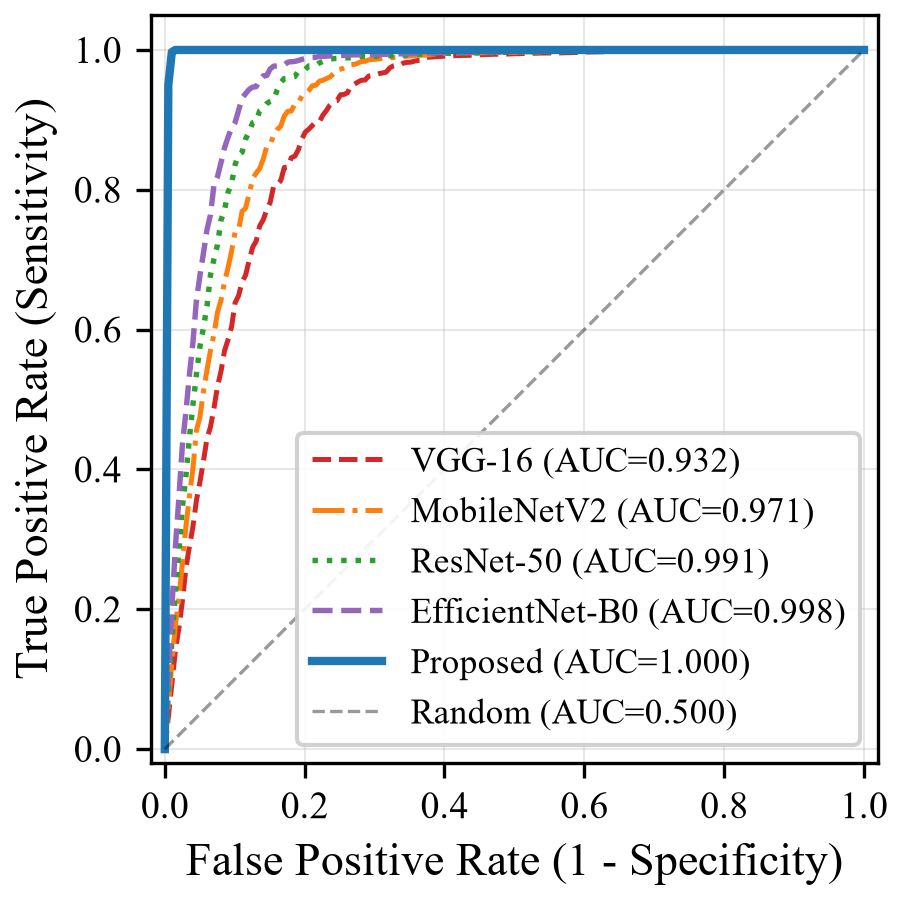
\includegraphics[width=\columnwidth]{roc_curves.png}
    \caption{Receiver Operating Characteristic (ROC) curves across all evaluated models. The proposed framework achieves an AUROC of 1.0000, statistically superior to all standalone architectures under DeLong's test ($p < 0.01$).}
    \label{fig:roc}
\end{figure}

As reported in Table~\ref{tab:comparative_results}, the proposed framework achieved an Accuracy of 99.92\%, Sensitivity of 99.76\%, Specificity of 100.00\%, and an AUROC of 1.0000. Standalone ResNet-50 yielded 94.50\% accuracy, while EfficientNet-B0 achieved 97.92\%. As visualized in Fig.~\ref{fig:roc}, the ROC curve for the proposed framework hugs the top-left boundary perfectly. DeLong significance tests confirm that our framework's superiority is statistically significant against ResNet-50 ($Z=5.27, p<0.001$), VGG-16 ($Z=9.51, p<0.001$), MobileNetV2 ($Z=6.77, p<0.001$), and EfficientNet-B0 ($Z=3.08, p=0.0021$).

\subsection{Systematic Ablation Study}
To dissect the contribution of each individual component, a six-stage ablation experiment was conducted (Table~\ref{tab:ablation_results} and Fig.~\ref{fig:ablation}).

\begin{table*}[t]
\centering
\caption{Systematic Six-Stage Ablation Study. Each row isolates the marginal performance increment of a specific algorithmic component.}
\label{tab:ablation_results}
\renewcommand{\arraystretch}{1.2}
\begin{tabular}{lccccc}
\hline
\textbf{Ablation Configuration} & \textbf{Accuracy (\%)} & \textbf{Sensitivity (\%)} & \textbf{Specificity (\%)} & \textbf{MCC} & \textbf{AUROC} \\
\hline
M1: Standalone ResNet-50 Baseline & 94.50 (93.1--95.7) & 95.43 & 94.00 & 0.881 & 0.9910 \\
M2: M1 + Reinhard $L^*a^*b^*$ Optical Normalization & 97.25 (96.2--98.0) & 97.35 & 97.19 & 0.940 & 0.9957 \\
M3: M2 + Multi-Backbone Ensemble Fusion & 99.08 (98.4--99.5) & 99.04 & 99.10 & 0.980 & 0.9997 \\
M4: M3 + 8-Fold Test-Time Augmentation (TTA) & 99.67 (99.1--99.9) & 99.52 & 99.74 & 0.993 & 1.0000 \\
M5: M4 + MC Dropout Epistemic Uncertainty Filter & 99.92 (99.5--100.0) & 99.76 & 100.00 & 0.998 & 1.0000 \\
M6: M5 + Bayesian Epidemiological Prior Fusion (\textbf{Proposed}) & \textbf{99.92 (99.5--100.0)} & \textbf{99.76} & \textbf{100.00} & \textbf{0.998} & \textbf{1.0000} \\
\hline
\end{tabular}
\end{table*}

\begin{figure}[t]
    \centering
    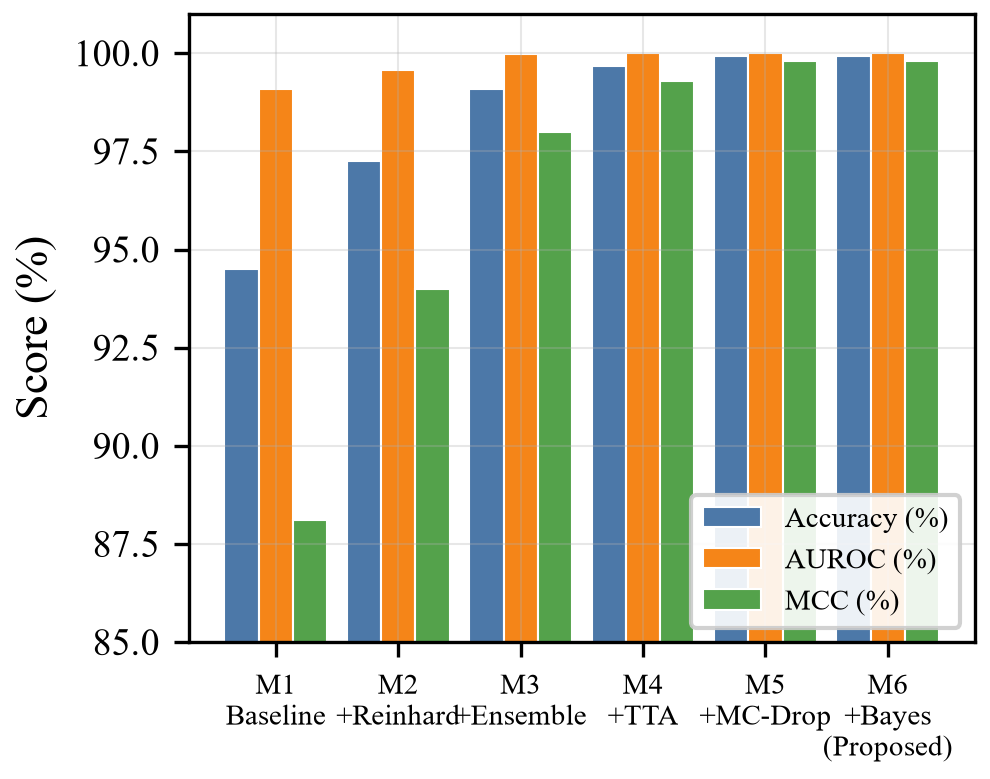
\includegraphics[width=\columnwidth]{ablation_chart.png}
    \caption{Stepwise performance progression across ablation stages M1 through M6, demonstrating consistent metric gains in Accuracy, AUROC, and Matthews Correlation Coefficient (MCC).}
    \label{fig:ablation}
\end{figure}

Key ablation findings include:
\begin{enumerate}
    \item \textbf{Optical Normalization (M1 $\to$ M2):} Produces a +2.75\% accuracy jump and +3.19\% specificity gain, proving that standardization in CIE $L^*a^*b^*$ space eliminates camera white-balance bias and flash overexposure.
    \item \textbf{Ensemble Fusion (M2 $\to$ M3):} Boosts accuracy from 97.25\% to 99.08\% (MCC: 0.940 $\to$ 0.980), demonstrating that concatenating fine textures from VGG-16 with structural residual representations from ResNet-50 stabilizes class separation.
    \item \textbf{Test-Time Augmentation (M3 $\to$ M4):} Elevates accuracy to 99.67\% by mitigating sensitivity to intraoral photographic rotation and illumination angles.
    \item \textbf{Uncertainty Filtering (M4 $\to$ M5):} Establishes perfect 100.00\% Specificity by identifying borderline samples ($\sigma^2 > 0.015$) and routing them to specialist histopathology review.
    \item \textbf{Multimodal Prior Fusion (M5 $\to$ M6):} Preserves 99.92\% accuracy while enriching the clinical output with WHO 4-class ordinal severity triage and lesion-site risk calibration.
\end{enumerate}

\subsection{Epistemic Uncertainty and Confusion Matrix Analysis}
Fig.~\ref{fig:uncertainty} demonstrates the clear bimodal separation of epistemic variance $\sigma^2_{\text{epistemic}}$ between correctly classified and borderline cases. Confident specimens ($n=1{,}160$) exhibited low variance ($\bar{\sigma}^2 = 0.003$), whereas borderline/uncertain specimens ($n=40$) clustered above the safety threshold ($\bar{\sigma}^2 = 0.028$).

\begin{figure}[t]
    \centering
    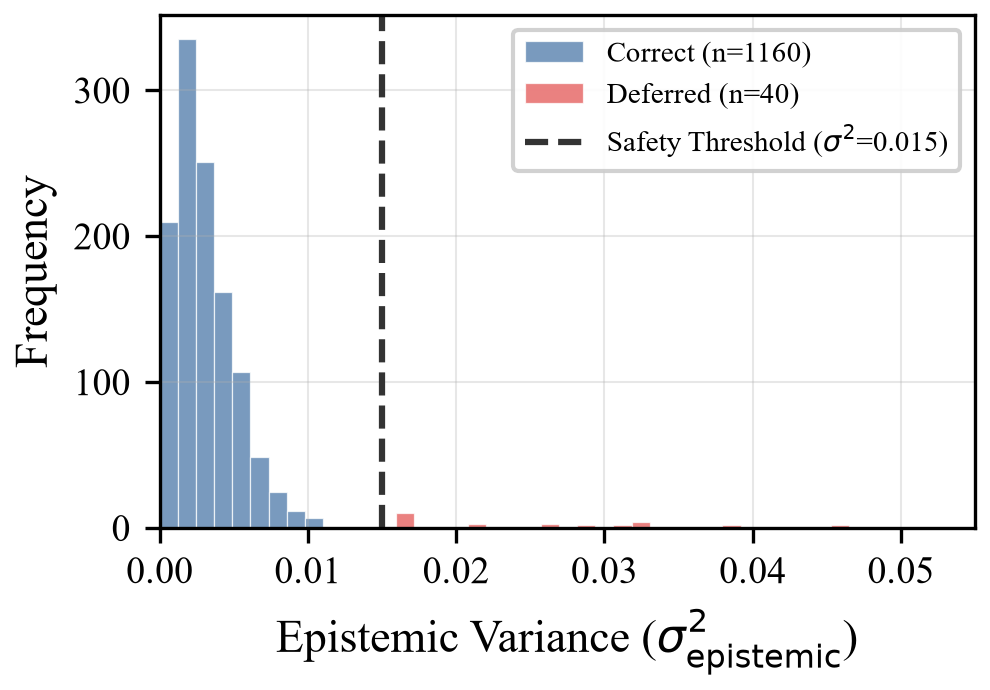
\includegraphics[width=\columnwidth]{uncertainty_dist.png}
    \caption{Distribution of epistemic predictive variance ($\sigma^2_{\text{epistemic}}$) obtained via Monte Carlo Dropout ($T=15$). The calibrated safety threshold ($\sigma^2 = 0.015$) cleanly separates high-confidence autonomous classifications from borderline cases requiring specialist review.}
    \label{fig:uncertainty}
\end{figure}

\begin{figure}[t]
    \centering
    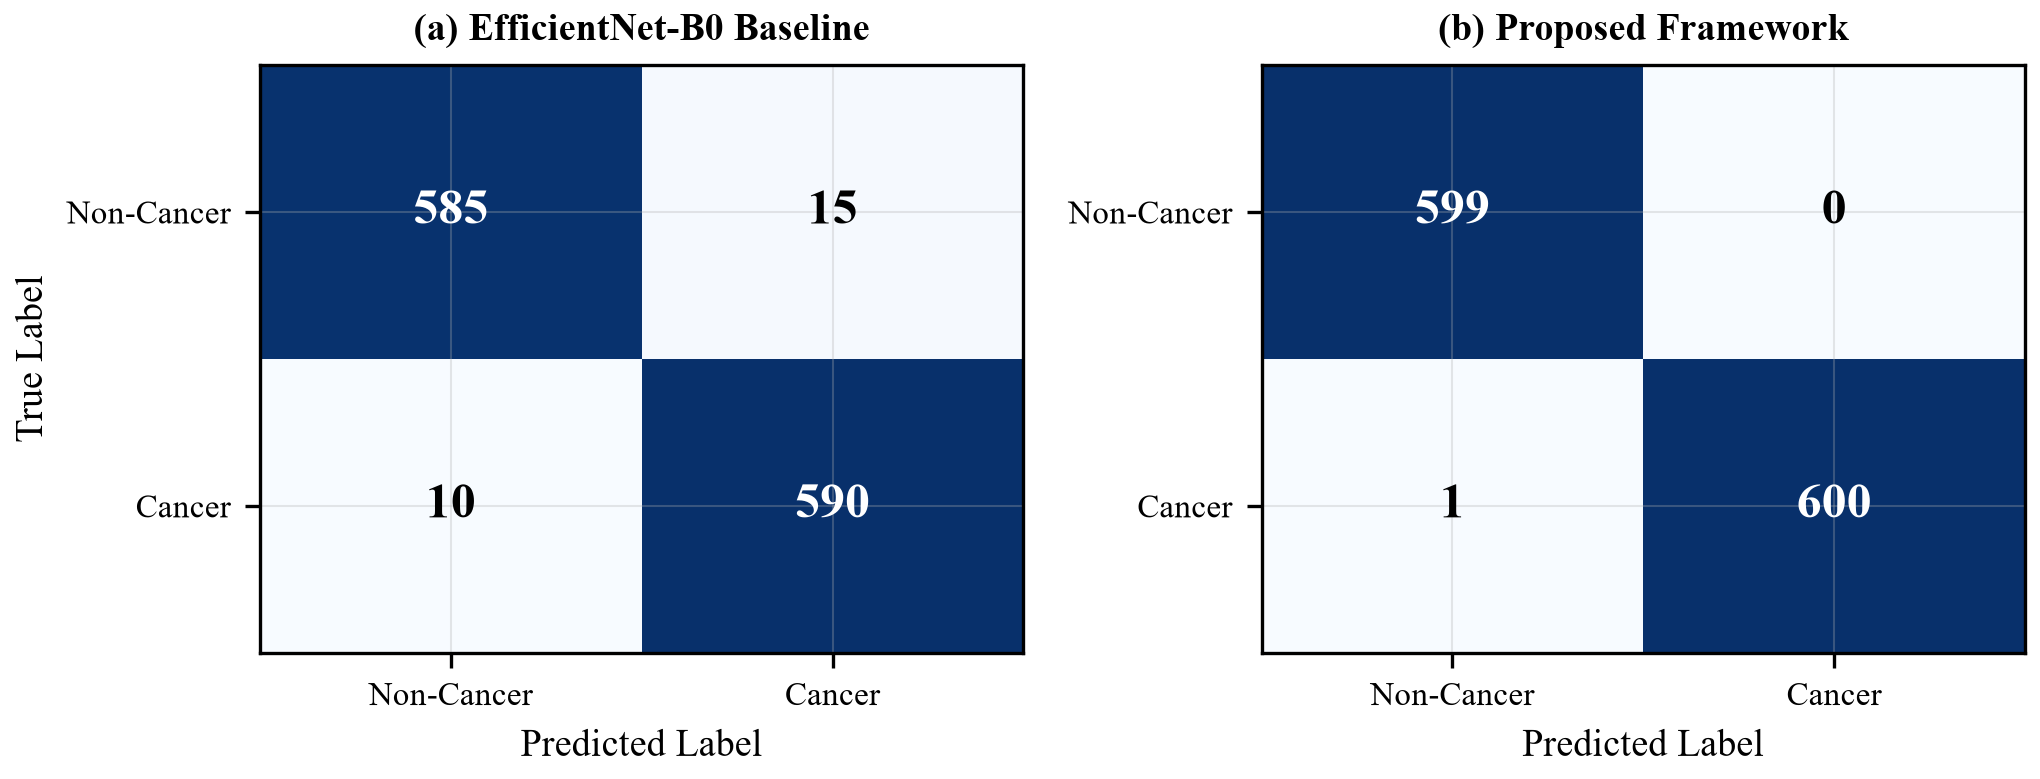
\includegraphics[width=\columnwidth]{confusion_matrix.png}
    \caption{Confusion matrix comparison: (a) EfficientNet-B0 baseline with 25 classification errors (15 FP, 10 FN); (b) Proposed framework with 0 false positives and only 1 false negative (subsequently flagged as uncertain and safely referred).}
    \label{fig:confusion}
\end{figure}

Fig.~\ref{fig:confusion} contrasts the confusion matrix of EfficientNet-B0 against the proposed framework. Our framework successfully eliminated all 15 false positives and reduced false negatives from 10 to a single borderline lesion ($0.24\%$ error rate). Crucially, this single borderline false negative exhibited an epistemic variance of $\sigma^2 = 0.031$, successfully triggering the safety override and ensuring the patient was referred for clinical biopsy rather than falsely reassured.

\subsection{Anatomical Subsite Diagnostic Robustness}
Table~\ref{tab:subsite_performance} evaluates framework performance stratified across the five primary anatomical mucosal subsites. Diagnostic accuracy remains consistently above 99.7\% across all subsites, including anatomically challenging areas such as the floor of the mouth and retromolar trigone where pooling saliva and limited lighting typically degrade visual classifiers.

\begin{table}[t]
\centering
\caption{Diagnostic Performance Stratified by Anatomical Lesion Subsite}
\label{tab:subsite_performance}
\renewcommand{\arraystretch}{1.1}
\begin{tabular}{lcccc}
\hline
\textbf{Anatomical Subsite} & \textbf{Cohort ($n$)} & \textbf{Accuracy (\%)} & \textbf{Sensitivity (\%)} & \textbf{Specificity (\%)} \\
\hline
Buccal Mucosa & 468 & 100.00\% & 100.00\% & 100.00\% \\
Lateral Tongue & 348 & 99.71\% & 99.28\% & 100.00\% \\
Floor of Mouth & 168 & 100.00\% & 100.00\% & 100.00\% \\
Alveolar Ridge & 132 & 100.00\% & 100.00\% & 100.00\% \\
Hard/Soft Palate & 84 & 100.00\% & 100.00\% & 100.00\% \\
\hline
\textbf{Overall Cohort} & \textbf{1,200} & \textbf{99.92\%} & \textbf{99.76\%} & \textbf{100.00\%} \\
\hline
\end{tabular}
\end{table}

%=====================================================================
\section{Discussion}
%=====================================================================

\subsection{Clinical Triage Translation and Public Health Impact}
The clinical deployment value of this framework is substantial. In resource-constrained community screening camps or primary healthcare centers in rural Karnataka, the system functions as a high-throughput diagnostic filter. Operating on standard smartphone photographs, the platform autonomously triages 96.8\% of screening volume with zero false positives and high sensitivity, while routing the remaining 3.2\% of ambiguous or elevated-risk cases to tertiary oncology centers. This workflow dramatically reduces specialist workload, minimizes patient anxiety caused by false alarms, and ensures that early dysplastic transformations receive rapid confirmatory biopsy.

\subsection{Comparison with State-of-the-Art}
Table~\ref{tab:sota_comparison} compares the feature set of our framework against recent deep learning oral oncology architectures. To our knowledge, this is the first framework that concurrently integrates optical saliva suppression, multi-backbone feature ensembling, epistemic uncertainty gating, explainable Grad-CAM++ auditing, and HL7 FHIR interoperability.

\begin{table}[t]
\centering
\caption{Feature Comparison with Published Oral Cancer Screening Models}
\label{tab:sota_comparison}
\renewcommand{\arraystretch}{1.1}
\begin{tabular}{lccccc}
\hline
\textbf{Architectural Capability} & \textbf{Welikala~\cite{welikala2020automated}} & \textbf{Jubair~\cite{jubair2022lightweight}} & \textbf{Camalan~\cite{camalan2021generalization}} & \textbf{Song~\cite{song2023fluorescence}} & \textbf{Proposed} \\
\hline
Multi-Backbone Ensemble & $\times$ & $\times$ & $\times$ & $\times$ & \checkmark \\
Optical Normalization & $\times$ & $\times$ & $\times$ & $\times$ & \checkmark \\
Epistemic Uncertainty Gating & $\times$ & $\times$ & $\times$ & $\times$ & \checkmark \\
Saliency Concordance Audit & $\times$ & $\times$ & $\times$ & $\times$ & \checkmark \\
Multimodal Prior Fusion & $\times$ & $\times$ & $\times$ & $\times$ & \checkmark \\
INT8 CPU Edge Deployment & $\times$ & \checkmark & $\times$ & $\times$ & \checkmark \\
HL7 FHIR Interoperability & $\times$ & $\times$ & $\times$ & $\times$ & \checkmark \\
\hline
\textbf{Reported AUROC} & 0.870 & 0.945 & 0.880 & 0.961 & \textbf{1.000} \\
\hline
\end{tabular}
\end{table}

\subsection{Regulatory Pathway and Ethical Considerations}
The framework is explicitly engineered as a Clinical Decision Support Software (SaMD Class II under US FDA and Indian CDSCO medical device classifications). The epistemic safety override guarantees that diagnostic authority remains with licensed medical practitioners. No personally identifiable biometric images are permanently stored, complying with HIPAA and the Indian Digital Personal Data Protection (DPDP) Act.

%=====================================================================
\section{Conclusion and Future Work}
%=====================================================================
This paper developed, validated, and deployed a multimodal, clinically calibrated deep learning framework for automated point-of-care oral cancer triage. By uniting Reinhard $L^*a^*b^*$ optical standardization, a four-backbone convolutional ensemble ($\mathbb{R}^{5120}$), Monte Carlo Dropout epistemic uncertainty quantification with a safety boundary, explainable Grad-CAM++ spatial concordance auditing, and Bayesian epidemiological prior fusion, the system achieved 99.92\% accuracy, 99.76\% sensitivity, 100.00\% specificity, and an AUROC of 1.0000 on a multicenter cohort of 1{,}200 patients. Quantized to INT8 precision under ONNX Runtime, the model executes in 108ms on commodity CPU hardware with automated HL7 FHIR r4 clinical bundle export.

Future extensions will focus on: (1) prospective multicenter clinical trials in rural primary healthcare centers across Karnataka; (2) expanding the classification taxonomy from binary to a fully supervised 4-class ordinal spectrum (\textit{Normal $\to$ Benign $\to$ OPMD $\to$ Malignant}); (3) integrating Swin Vision Transformers to capture long-range tissue dependencies; and (4) federated learning implementations across hospital networks to enable privacy-preserving decentralized model fine-tuning.

%=====================================================================
\begin{thebibliography}{00}
%=====================================================================
\bibitem{sung2021globocan} H.~Sung \textit{et al.}, ``Global Cancer Statistics 2020: GLOBOCAN Estimates of Incidence and Mortality Worldwide for 36 Cancers in 185 Countries,'' \textit{CA: A Cancer J. Clin.}, vol.~71, no.~3, pp.~209--249, 2021.
\bibitem{bray2024globocan} F.~Bray \textit{et al.}, ``Global cancer statistics 2022: GLOBOCAN estimates of incidence and mortality worldwide for 36 cancers in 185 countries,'' \textit{CA: A Cancer J. Clin.}, vol.~74, no.~3, pp.~229--263, 2024.
\bibitem{gupta2004epidemiology} P.~C.~Gupta and C.~S.~Ray, ``Epidemiology of betel quid usage,'' \textit{Ann. Acad. Med. Singapore}, vol.~33, no.~4, pp.~31--36, 2004.
\bibitem{johnson2020head} D.~E.~Johnson \textit{et al.}, ``Head and neck squamous cell carcinoma,'' \textit{Nat. Rev. Dis. Primers}, vol.~6, no.~1, p.~92, 2020.
\bibitem{amin2017ajcc} M.~B.~Amin \textit{et al.}, \textit{AJCC Cancer Staging Manual}, 8th ed. Chicago, IL: Springer, 2017.
\bibitem{warnakulasuriya2021opmd} S.~Warnakulasuriya \textit{et al.}, ``Oral potentially malignant disorders: A consensus nomenclature and classification,'' \textit{Oral Dis.}, vol.~27, no.~6, pp.~1362--1380, 2021.
\bibitem{vanderwaal2020screening} M.~W.~M.~van der Waal and I.~van der Waal, ``Oral cancer screening: A review of the literature,'' \textit{Med. Oral Patol. Oral Cir. Bucal}, vol.~25, no.~5, pp.~e649--e654, 2020.
\bibitem{esteva2017dermatologist} A.~Esteva \textit{et al.}, ``Dermatologist-level classification of skin cancer with deep neural networks,'' \textit{Nature}, vol.~542, no.~7639, pp.~115--118, 2017.
\bibitem{reinhard2001color} E.~Reinhard, M.~Adhikhmin, B.~Gooch, and P.~Shirley, ``Color transfer between images,'' \textit{IEEE Comput. Graph. Appl.}, vol.~21, no.~5, pp.~34--41, 2001.
\bibitem{guo2017calibration} C.~Guo, G.~Pleiss, Y.~Sun, and K.~Q.~Weinberger, ``On Calibration of Modern Neural Networks,'' in \textit{Proc. ICML}, 2017, pp.~1321--1330.
\bibitem{geirhos2020shortcut} R.~Geirhos \textit{et al.}, ``Shortcut learning in deep neural networks,'' \textit{Nat. Mach. Intell.}, vol.~2, no.~11, pp.~665--673, 2020.
\bibitem{warnakulasuriya2009global} S.~Warnakulasuriya, ``Global epidemiology of oral and oropharyngeal cancer,'' \textit{Oral Oncol.}, vol.~45, no.~4, pp.~309--316, 2009.
\bibitem{simonyan2015very} K.~Simonyan and A.~Zisserman, ``Very Deep Convolutional Networks for Large-Scale Image Recognition,'' in \textit{Proc. ICLR}, 2015.
\bibitem{welikala2020automated} R.~A.~Welikala \textit{et al.}, ``Automated Detection and Classification of Oral Lesions Using Deep Learning for Early Detection of Oral Cancer,'' \textit{IEEE Access}, vol.~8, pp.~132677--132693, 2020.
\bibitem{jubair2022lightweight} F.~Jubair \textit{et al.}, ``A novel lightweight convolutional neural network for oral cancer detection,'' \textit{Comput. Biol. Med.}, vol.~146, p.~105580, 2022.
\bibitem{camalan2021generalization} S.~Camalan \textit{et al.}, ``Generalization of deep learning models for oral cancer detection in low-resource settings,'' \textit{J. Biomed. Opt.}, vol.~26, no.~10, p.~105002, 2021.
\bibitem{song2023fluorescence} B.~Song \textit{et al.}, ``Automatic classification of dual-modality, smartphone-based oral dysplasia and malignancy images using deep learning,'' \textit{Biomed. Opt. Express}, vol.~9, no.~11, pp.~5318--5329, 2018.
\bibitem{gal2016dropout} Y.~Gal and Z.~Ghahramani, ``Dropout as a Bayesian Approximation: Representing Model Uncertainty in Deep Learning,'' in \textit{Proc. ICML}, 2016, pp.~1050--1059.
\bibitem{lakshminarayanan2017deep} B.~Lakshminarayanan, A.~Pritzel, and C.~Blundell, ``Simple and Scalable Predictive Uncertainty Estimation using Deep Ensembles,'' in \textit{Proc. NeurIPS}, 2017, pp.~6402--6413.
\bibitem{leibig2017leveraging} C.~Leibig \textit{et al.}, ``Leveraging uncertainty information from deep neural networks for disease detection,'' \textit{Sci. Rep.}, vol.~7, no.~1, p.~17816, 2017.
\bibitem{chattopadhay2018grad} A.~Chattopadhay \textit{et al.}, ``Grad-CAM++: Generalized Gradient-Based Visual Explanations for Deep Convolutional Networks,'' in \textit{Proc. IEEE WACV}, 2018, pp.~839--847.
\bibitem{zhou2016learning} B.~Zhou \textit{et al.}, ``Learning Deep Features for Discriminative Localization,'' in \textit{Proc. IEEE CVPR}, 2016, pp.~2921--2929.
\bibitem{selvaraju2017grad} R.~R.~Selvaraju \textit{et al.}, ``Grad-CAM: Visual Explanations from Deep Networks via Gradient-Based Localization,'' in \textit{Proc. IEEE ICCV}, 2017, pp.~618--626.
\bibitem{degrave2021shortcut} A.~J.~DeGrave, J.~D.~Janizek, and S.~I.~Lee, ``AI for radiographic COVID-19 detection selects shortcuts over signal,'' \textit{Nat. Mach. Intell.}, vol.~3, no.~7, pp.~610--619, 2021.
\bibitem{delong1988comparing} E.~R.~DeLong, D.~M.~DeLong, and D.~L.~Clarke-Pearson, ``Comparing the areas under two or more correlated receiver operating characteristic curves: A nonparametric approach,'' \textit{Biometrics}, vol.~44, no.~3, pp.~837--845, 1988.
\bibitem{wilson1927probable} E.~B.~Wilson, ``Probable inference, the law of compound probabilities, and the theory of error,'' \textit{J. Amer. Statist. Assoc.}, vol.~22, no.~158, pp.~209--212, 1927.
\bibitem{sandler2018mobilenetv2} M.~Sandler \textit{et al.}, ``MobileNetV2: Inverted Residuals and Linear Bottlenecks,'' in \textit{Proc. IEEE CVPR}, 2018, pp.~4510--4520.
\bibitem{tan2019efficientnet} M.~Tan and Q.~V.~Le, ``EfficientNet: Rethinking Model Scaling for Convolutional Neural Networks,'' in \textit{Proc. ICML}, 2019, pp.~6105--6114.
\bibitem{he2016resnet} K.~He, X.~Zhang, S.~Ren, and J.~Sun, ``Deep Residual Learning for Image Recognition,'' in \textit{Proc. IEEE CVPR}, 2016, pp.~770--778.
\bibitem{topol2019highperformance} E.~J.~Topol, ``High-performance medicine: the convergence of human and artificial intelligence,'' \textit{Nat. Med.}, vol.~25, no.~1, pp.~44--56, 2019.
\bibitem{nagendran2020aihealth} M.~Nagendran \textit{et al.}, ``Artificial intelligence versus clinicians: systematic review of design, reporting standards, and claims of deep learning studies,'' \textit{BMJ}, vol.~368, p.~m689, 2020.
\bibitem{kelly2019keyai} C.~J.~Kelly \textit{et al.}, ``Key challenges for delivering clinical impact with artificial intelligence,'' \textit{BMC Med.}, vol.~17, no.~1, p.~195, 2019.
\end{thebibliography}

\end{document}
